\documentclass{article}
\usepackage{rotating}

\usepackage{tikz}
\usepackage{graphicx}
\usepackage{fontspec}
\usepackage{tocloft}
\usepackage{titletoc}
\usepackage{lipsum}
\usepackage{titlesec}

\setcounter{secnumdepth}{4}


\setmainfont{OpenSans-VariableFont_wdth,wght.ttf}[Path=assets/]

\begin{document}
%%%%%%%%%%    COVER    %%%%%%%%%%
\begin{titlepage}

\begin{flushright}

\vspace{7.5cm}

\Huge Team 1 EN.605.204.81 \\ ARM32 RSA Design Document V2

\vspace{0.5cm}

\Large Rohan Abraham, Tero Suontaka, Sullivan Prellwitz

\vspace{8cm}

\normalsize April 28, 2024

\end{flushright}

\end{titlepage}
\newpage
%%%%%%%%%%%%%%%%%%%%%%%%%%%%%%%%%
%%%%%%%%%%    LIST OF CONTENTS    %%%%%%%%%%
\tableofcontents
\newpage
%%%%%%%%%%%%%%%%%%%%%%%%%%%%%%%%%
%%%%%%%%%%    CONTENT    %%%%%%%%%%
\setmainfont{OpenSans-VariableFont_wdth,wght.ttf}[Path=assets/]
\section{Goals}
\setmainfont{OpenSans-VariableFont_wdth,wght.ttf}[Path=assets/]
Purpose: Encrypt and decrypt messages using a custom RSA implementation in ARM32 assembly.
Implement a modular design for all functions and create a library of assembly code that enables the generation of a public and private RSA keys using user specified values.
\newpage

\setmainfont{OpenSans-VariableFont_wdth,wght.ttf}[Path=assets/]
\section{Architecture}
\setmainfont{OpenSans-VariableFont_wdth,wght.ttf}[Path=assets/]
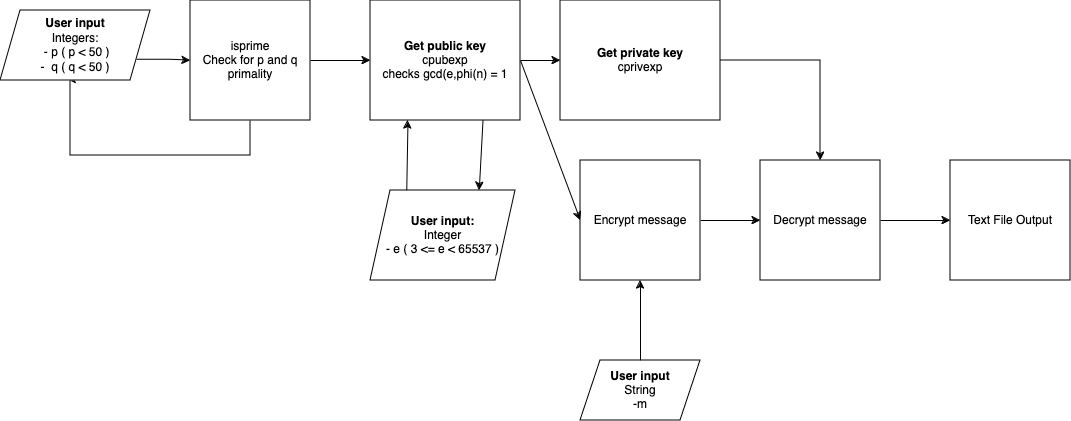
\includegraphics[scale=0.44]{assets/rsa-impl.drawio.png}
\section{Functions}
\setmainfont{OpenSans-VariableFont_wdth,wght.ttf}[Path=assets/]
    \subsection{libIO.s}
        \subsubsection{stringToArray}
        \paragraph*{Purpose:}
            {Converts a string (byte array) to an array of 32 bit integers \\ }
            input:\begin{itemize}
                \item r0 - pointer to string
                \item r1 - size of string
            \end{itemize}
            Output:\begin{itemize}
                \item r0 - pointer to integer
                \item r1 - size of array
            \end{itemize}
            
        \subsubsection{arrayToString}
        \paragraph*{Purpose:}
            {Converts an integer array to a null delimited string \\ }
            input:\begin{itemize}
                \item r0 - pointer to integer array
                \item r1 - size of array
            \end{itemize}
            Output:\begin{itemize}
                \item r0 - pointer to string
                \item r1 - size of string
            \end{itemize}

        \subsubsection{writeFile}
        \paragraph*{Purpose:}
            {Write to a file, name provided by user \\ }
            input:\begin{itemize}
                \item r0 - name of file to write
                \item r1 - pointer to message to write
            \end{itemize}
            
        \subsubsection{writeArray}
        \paragraph*{Purpose:}
            {Write 32 bit integer array to a file \\ }
            input:\begin{itemize}
                \item r0 - pointer to string
                \item r1 - pointer to message to write
                \item r2 - length of string
            \end{itemize}

        \subsubsection{readArray}
        \paragraph*{Purpose:}
            {Read file to 32 bit integer array \\ }
            input:\begin{itemize}
                \item r0 - name of file to read
            \end{itemize}
            Output:\begin{itemize}
                \item r0 - pointer to array
                \item r1 - array length
            \end{itemize}
    \subsection{libMath.s}
        \subsubsection{gcd}
            \paragraph*{Purpose:}
                {Computes the greatest common divisor of two integers \\ }
                input:\begin{itemize}
                    \item r0 - first integer to compute gcd of
                    \item r1 - second integer to compute gcd of
                \end{itemize}
                Output:\begin{itemize}
                    \item r0 - greatest common divisor of two input integers
                \end{itemize}
        \subsubsection{mod}
            \paragraph*{Purpose:}
                {Modulo calculation: r0 mod r1 = r0 \\ }
                input:\begin{itemize}
                    \item r0 - first integer to compute modulo
                    \item r1 - second integer to compute modulo
                \end{itemize}
                Output:\begin{itemize}
                    \item r0 - modulo value
                \end{itemize}
        \subsubsection{isPrime}
            \paragraph*{Purpose:}
                {Determines if a number is prime \\ }
                input:\begin{itemize}
                    \item r0 - integer to test
                \end{itemize}
                Output:\begin{itemize}
                    \item r0 - binary value indicating primality returns -1 for invalid values
                \end{itemize}
        \subsubsection{totient}
            \paragraph*{Purpose:}
                {Totient calculation Φ(n) = (p – 1) (q – 1) s.t. p and q are prime \\ }
                input:\begin{itemize}
                    \item r0 - p
                    \item r1 - q
                \end{itemize}
                Output:\begin{itemize}
                    \item r0 - return: totient value of (n) or r0 == -1 if p or q are NOT prime (error)
                \end{itemize}
    \subsection{libRSA.s}
        \subsubsection{cprivexp}
            \paragraph*{Purpose:}
                {Calculates the private exponent. Calculates multiplicative inverse of public key over ring of integers mod n \\}
                input:\begin{itemize}
                    \item r0 - public exponent (e)
                    \item r1 - integer such that gcd(r0,r1) = 1 (phi(n))
                \end{itemize}
                Output:\begin{itemize}
                    \item r0 - private exponent returns -1 if gcd(r0,r1) != 1
                \end{itemize}
        \subsubsection{cpubexp}
            \paragraph*{Purpose:}
                {Validates the public exponent s.t. 1 < e < Φ(n) and e is co-prime to Φ(n) [ gcd(e, Φ(n)) = 1 ] \\}
                input:\begin{itemize}
                    \item r0 - p
                    \item r1 - q
                    \item r2 - e
                \end{itemize}
                Output:\begin{itemize}
                    \item r0 - pub exponent or -1 if error
                \end{itemize}
        \subsubsection{process}
            \paragraph*{Purpose:}
                {Processes the input for RSA encryption and decryption. For encryption, use private key as exponent. For decryption, use public key as exponent \\}
                input:\begin{itemize}
                    \item r0 - integer base a
                    \item r1 - integer exponent b
                    \item r2 - integer modulus n
                \end{itemize}
                Output:\begin{itemize}
                    \item r0 - a \^{}  b mod n
                \end{itemize}
        \subsubsection{processArray}
            \paragraph*{Purpose:}
                {Processes an integer array for RSA encryption and decryption. Applies a\^{}b mod n for all a in array. \\}
                input:\begin{itemize}
                    \item r0 - pointer to integer array
                    \item r1 - size of array
                    \item r2 - integer exponent b
                    \item r3 - integer modulus n
                \end{itemize}
                Output:\begin{itemize}
                    \item r0 - pointer to processed integer array
                    \item r1 - size of array
                \end{itemize}

        \subsubsection{generateKeys}
            \paragraph*{Purpose:}
                {Prompt user for primes and public exponent and generate private key \\}

        \subsubsection{encrypt}
            \paragraph*{Purpose:}
                {Encrypts a message given user input public key and modulus and writes to encrypted.txt \\}
        \subsubsection{decrypt}
            \paragraph*{Purpose:}
                {Decrypts a message from encrypted.txt given user input private key and modulus and writes plaintext to plaintext.txt\\}
        
    \subsection{main.s}
        \subsubsection{main}
        \paragraph*{Purpose:}
                {Drives the generation of keys, encryption, and decryption }
\newpage

\setmainfont{OpenSans-VariableFont_wdth,wght.ttf}[Path=assets/]
\section{Testability}
\setmainfont{OpenSans-VariableFont_wdth,wght.ttf}[Path=assets/]
    To facilitate easy testing the majority of functions are called directly in the Rust project located
    in the \verb|/tests| directory. This project is made up of three main parts:
    \begin{enumerate}
        \item \verb|lib.rs| - the test library in rust
        \item \verb|testHelper.s| - an arm assembly helper file for the test library
        \item \verb|Makefile| - the Makefile is responsible for building and linking all related assembly code to a shared library  \verb|libRSA.so|
    \end{enumerate}
    \subsection{Notes on the test project:}
    \begin{itemize}
        \item Throughout the test project a public key, private key, and modulus value that are referenced. These values are as follows:
        \begin{itemize}
            \item \verb|pubkey: 557|
            \item \verb|privkey: 1493|
            \item \verb|mod: 1763|
        \end{itemize}
        \item Text files created by the test project will live within the \verb|test/| directory
        \item For tests using a plaintext the string used is \verb|hello plaintext|
        \item For tests using an array version of the plaintext the string remains the same and the array values are base 10 integers representing character ASCII value
        \item For tests using a ciphertext the array values provided in the tests are derived from the above plaintext, pub/priv key, and mod values
        \item To circumvent problems with memory management and lifetime all arrays are dealt with through files to ensure correctness
        \item For information on compiling and running the tests please see the \verb|README.md| in the \verb|test/| directory
    \end{itemize}
    
\newpage

\setmainfont{OpenSans-VariableFont_wdth,wght.ttf}[Path=assets/]
\section{Timeline}
\setmainfont{OpenSans-VariableFont_wdth,wght.ttf}[Path=assets/]
    \subsection{March 11 - 15}
        \begin{itemize}
            \item First implementation meeting
            \item Initialize code repository
            \item mod function implementation finished, tests written
        \end{itemize}
    \subsection{March 25 - 29}
         \begin{itemize}
            \item Second implementation meeting
            \item gcd, pow, and tot implementation finished, tests written
            \item Plan next implementation steps
        \end{itemize}
    \subsection{April 8 - 20}
        \begin{itemize}
            \item Meet as needed
            \item RSA implementation finished (April 20), tests written
            \item Creation of testing control script
        \end{itemize}
    \subsection{April 21 - 27}
        \begin{itemize}
            \item Complete testing
            \item Squash bugs
            \item Prep repository and extra materials for submission
        \end{itemize}
    \subsection{April 28}
        \begin{itemize}
            \item Submit implementation
        \end{itemize}
\newpage

\section{Screenshots}
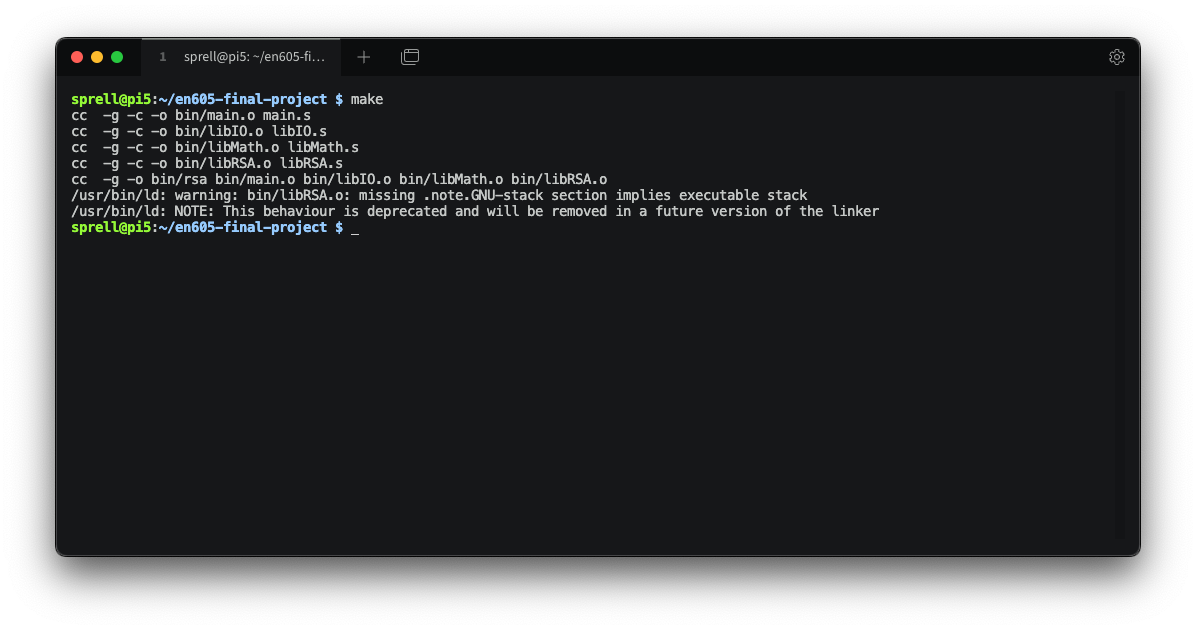
\includegraphics[scale=0.40]{assets/make-proj.png}
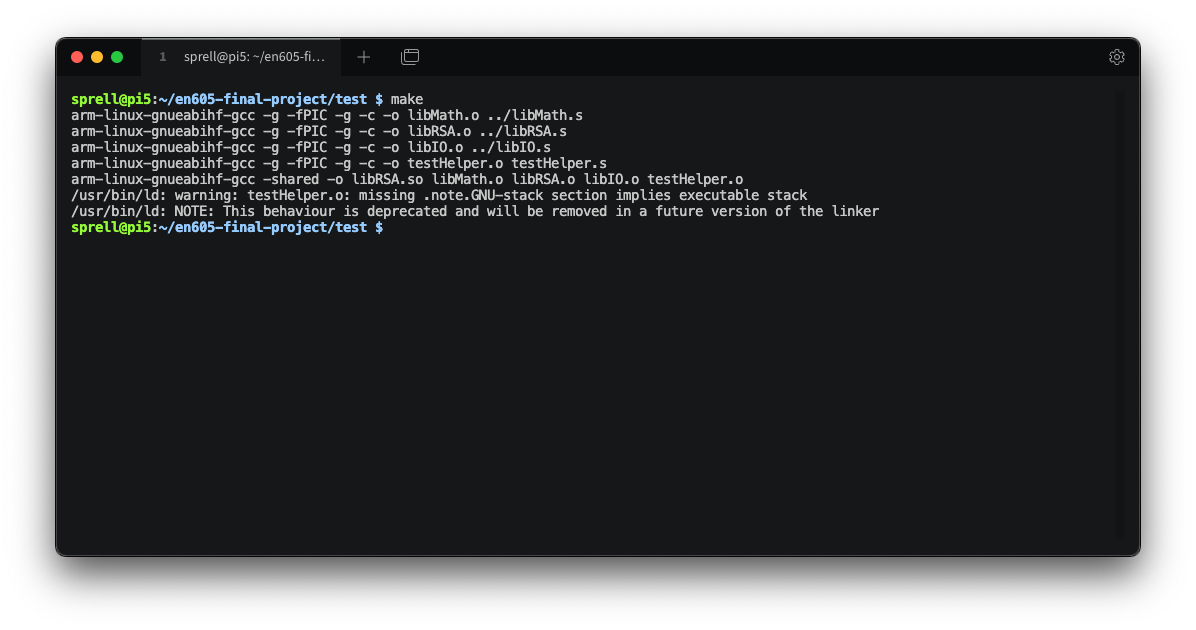
\includegraphics[scale=0.40]{assets/make-test.png}
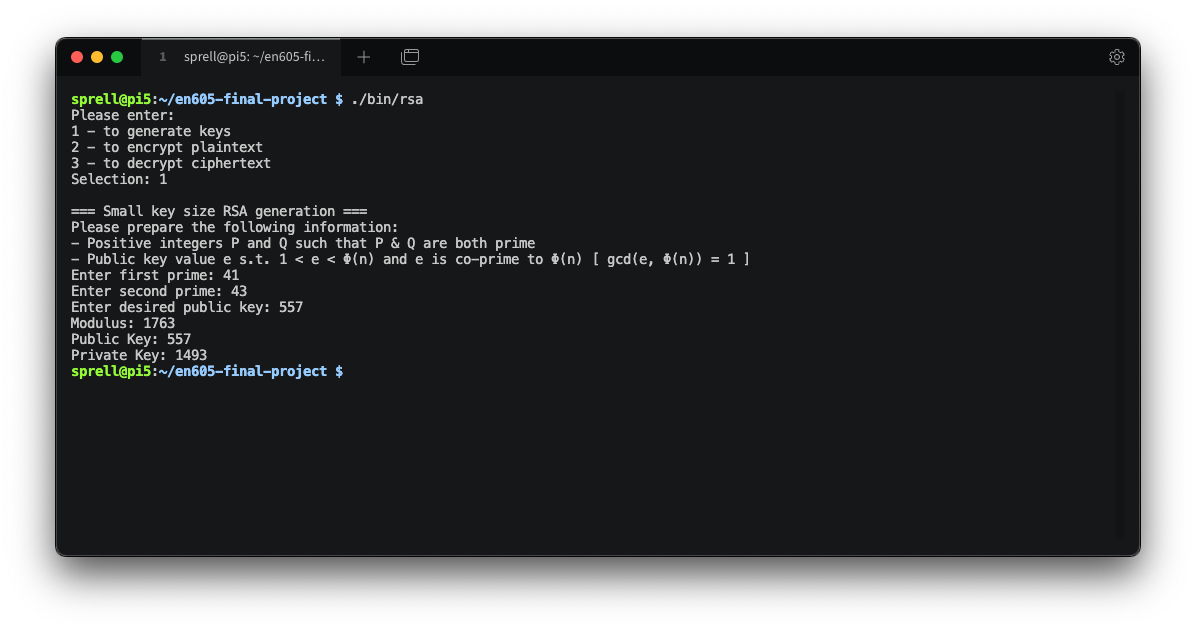
\includegraphics[scale=0.40]{assets/keygen.png}
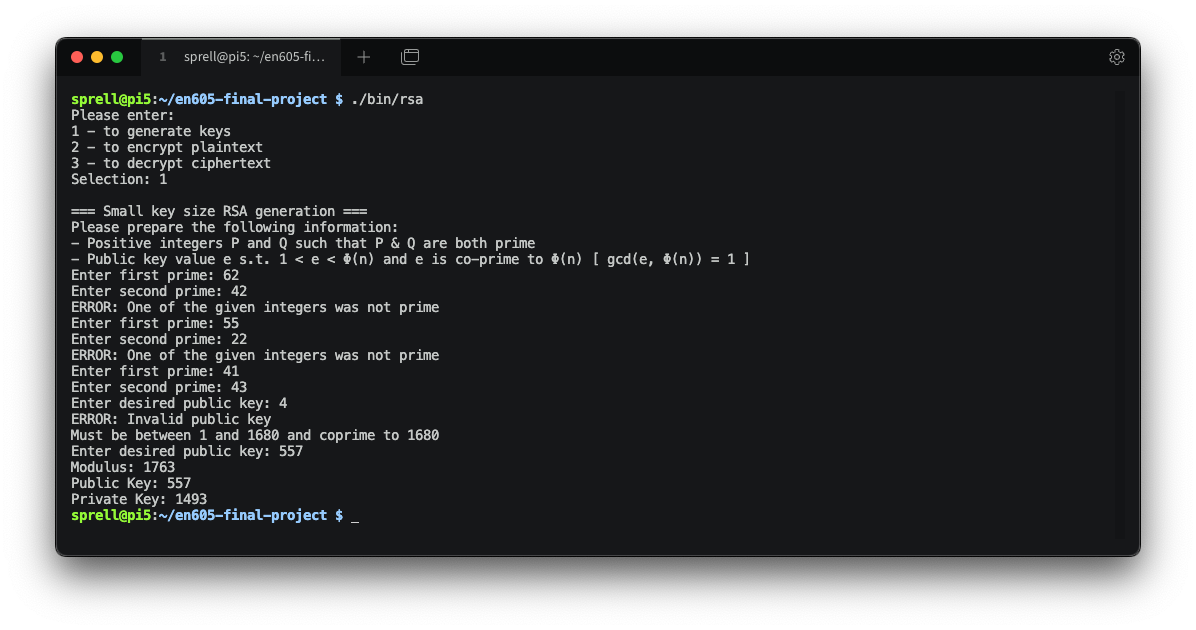
\includegraphics[scale=0.40]{assets/keygen-werr.png}
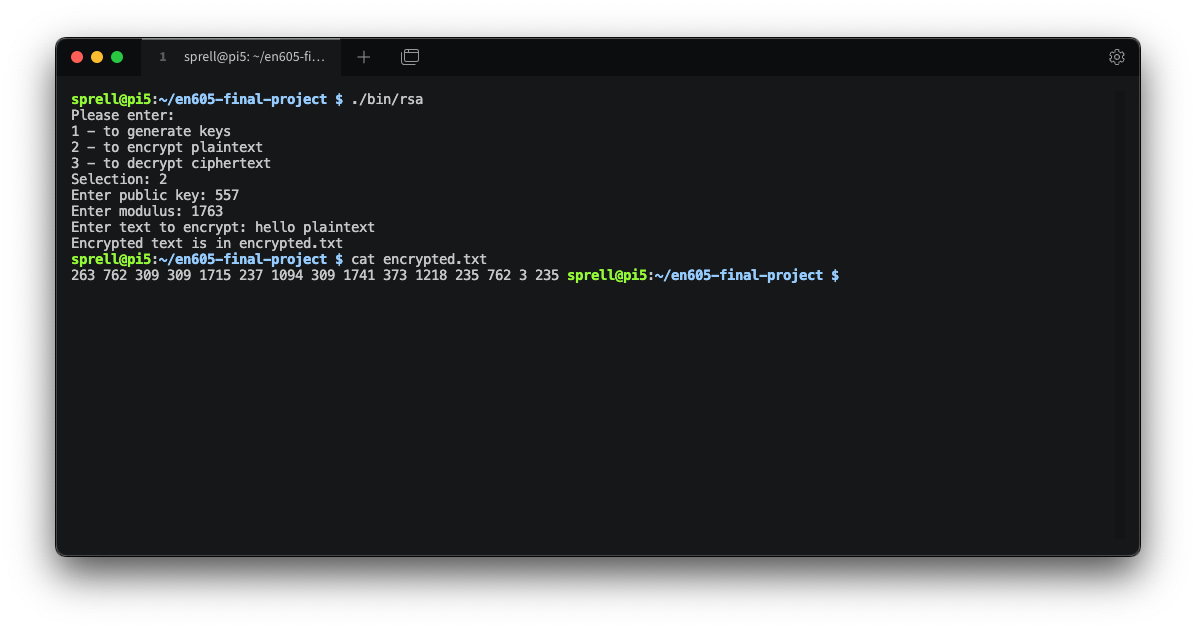
\includegraphics[scale=0.40]{assets/encrypt.png}
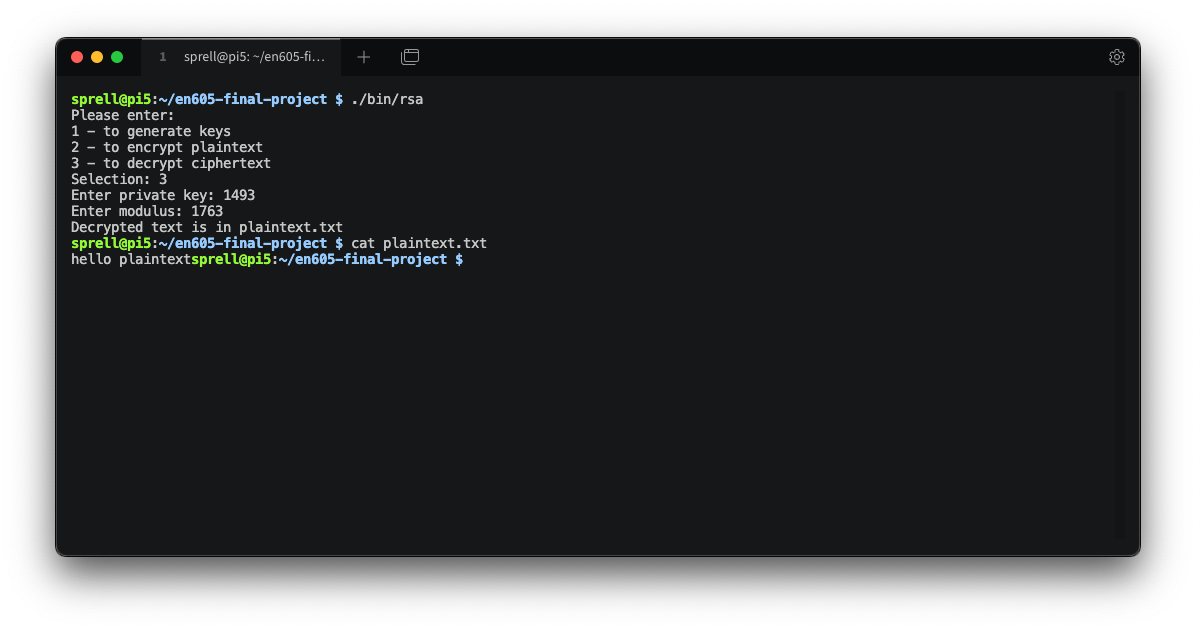
\includegraphics[scale=0.40]{assets/decrypt.png}
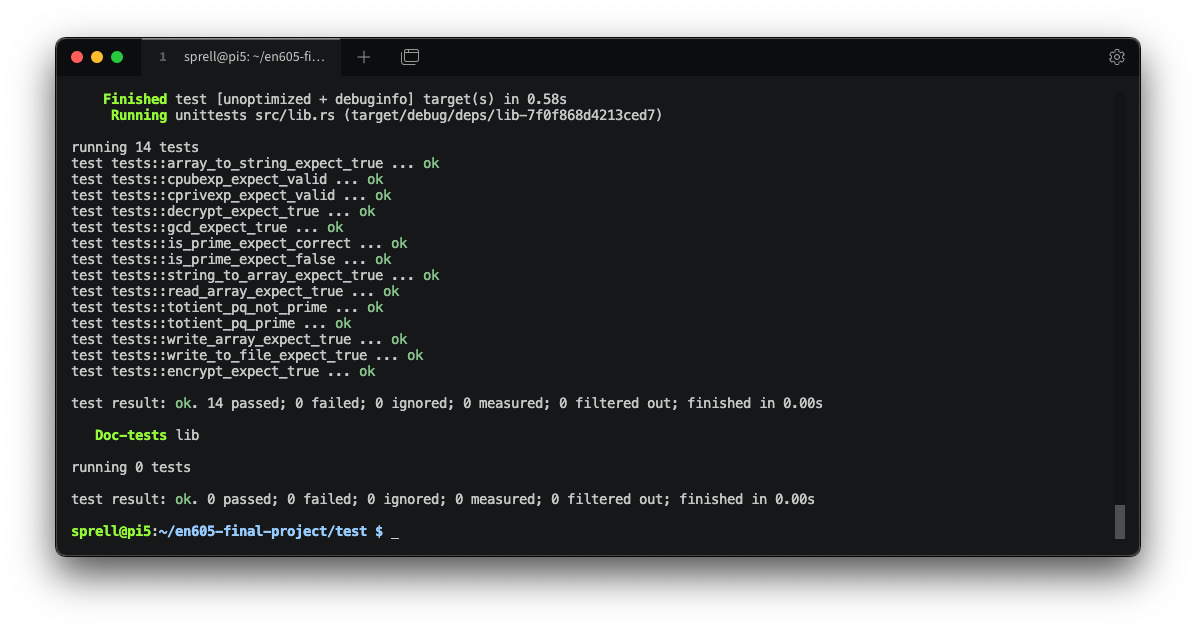
\includegraphics[scale=0.40]{assets/rust-tests.png}

%%%%%%%%%%%%%%%%%%%%%%%%%%%%%%%%%
\end{document}

\begin{comment}

\end{comment}